%********************************************************************************************
%								COMANDOS ÚTILES PARA LATEX EN ESTE TP							
%
%	\ : espacio simple
%	\\ : nueva línea
%	\par : va a la línea de abajo y deja sangría
%	\vspace{##tamaño en pt##} o \vspace{\baselineskip} en general:
%								 para dejar un espacio vertical
%	\textbf{text} :text en negrita
%	\textit{text} :text en itálica
%
% GRAFICOS CENTRADOS:
%	\begin{center}
%		\includegraphics[width=\textwidth]{./img/##ruta imagen (no hace falta extension)##}
%	\end{center}
%		--> se pueden agregar atributos como scale por si se hace muy grande
%
% TABLAS CENTRADAS:
%	\begin{center}
%	\begin{tabular}{|c|c|}
%	\hline
%	\ \textbf{Programa} & \textbf{Ticks} \\
%	\hline
%		ASM & 675127609 \\
%	\hline
%	\end{tabular}
%	\end{center}
%
% ALGORITMOS (EN VARIOS LENGUAJES):
% \begin{lstlisting}
%	void sumoDiez(int &num)
%	{
%	    num += 10;
%	}
%	
%	int main()
%	{
% 	   int i;
%	    int numeroAProcesar = 20;
%	    for (i = 0; i < 50; i++)
%	    {
%	        sumoDiez(numeroAProcesar);	//Proceso el numero en cada ciclo
%	    } 
%	    return 0;
%	}
%	\end{lstlisting}
%
% para info sobre todo lo que tiene el package detallado:
% http://en.wikibooks.org/wiki/LaTeX/Source\_Code\_Listings
%
%********************************************************************************************

\documentclass[10pt,a4paper]{article}
\usepackage[utf8]{inputenc} % para poder usar tildes en archivos UTF-8
\usepackage[spanish]{babel} % para que comandos como \today den el resultado en castellano
\usepackage{a4wide} % márgenes un poco más anchos que lo usual
\usepackage[conEntregas]{caratula}
\usepackage{amssymb}
\usepackage{fancybox}
\usepackage[usenames,dvipsnames]{color}
\usepackage{hyperref}
\usepackage{listings}
\usepackage{ulem}
\usepackage{color}
\usepackage[table]{xcolor}
\usepackage{amsmath}
\usepackage{float}
\usepackage{pdflscape}
%\usepackage[landscape]{geometry}

\hypersetup{
    colorlinks,
    citecolor=black,
    filecolor=black,
    linkcolor=black,
    urlcolor=black
}

\lstdefinestyle{customc}{
  belowcaptionskip=1\baselineskip,
  breaklines=true,
  frame=L,
  xleftmargin=\parindent,
  language=C,
  showstringspaces=false,
  basicstyle=\footnotesize\ttfamily,
  keywordstyle=\bfseries\color{green!40!black},
  commentstyle=\itshape\color{purple!40!black},
  identifierstyle=\color{blue},
  stringstyle=\color{orange},
}

\lstset{escapechar=@,style=customc, language=SQL}


\newcommand{\pk}[1]{\textbf{\textcolor{PineGreen}{\underline{{#1}}}}}

\newcommand{\fk}[1]{\textbf{\textcolor{red}{\dashuline{{#1}}}}}
\newcommand{\nullableFk}[1]{\textbf{\textcolor{YellowOrange}{\dashuline{{#1}}}}}

\newcommand{\nullableAtribute}[1]{\textbf{\textcolor{MidnightBlue}{{#1}}}}

\begin{document}

\titulo{Trabajo Práctico 1}
%\subtitulo{}

\fecha{\today}

\materia{Bases de Datos}
\grupo{Grupo 5}

\integrante{Barbeiton, Nicolás}{147/10}{nicolasbarbeiton@gmail.com}
\integrante{Chapresto, Matias Nahuel}{201/12}{matiaschapresto@gmail.com}
\integrante{Garassino, Agustín Javier}{394/12}{ajgarassino@gmail.com}
\integrante{Vileriño, Silvio}{106/12}{svilerino@gmail.com}

\maketitle

\tableofcontents
\newpage

\section{Introducción}
%ya esta el section en informe.tex
%\section{Introducción}
El objetivo de este trabajo practico es el diseño e implementacion de una solucion que satisfaga los requerimientos del cliente. En esta ocasion se nos requiere un sistema que permita implementar el \texttt{Voto Electronico} en Elecciones. Para ello, teniendo como base un relevamiento del problema -enunciado-, realizaremos un diagrama de entidad relacion y especificaremos restricciones adicionales que este modelo no capture. Como siguiente paso, derivaremos de un modelo relacional. Teniendo como base el modelo relacional, lo implementaremos en un motor de base de datos propietario, creando las tablas, claves y relaciones adecuadas. Adicionalmente, para satisfacer ciertas restricciones y proveer operaciones consistentes, necesitaremos implementar \texttt{triggers}, \texttt{stores procedures} y \texttt{constraint checks} sobre el motor fisico. Finalmente, proveeremos una suite adecuada de tests que verifiquen la robustez del sistema construido. 

\section{Desarrollo}
\subsection{Diagrama Entidad-Relacion}
	\begin{figure}
	  \centering	
		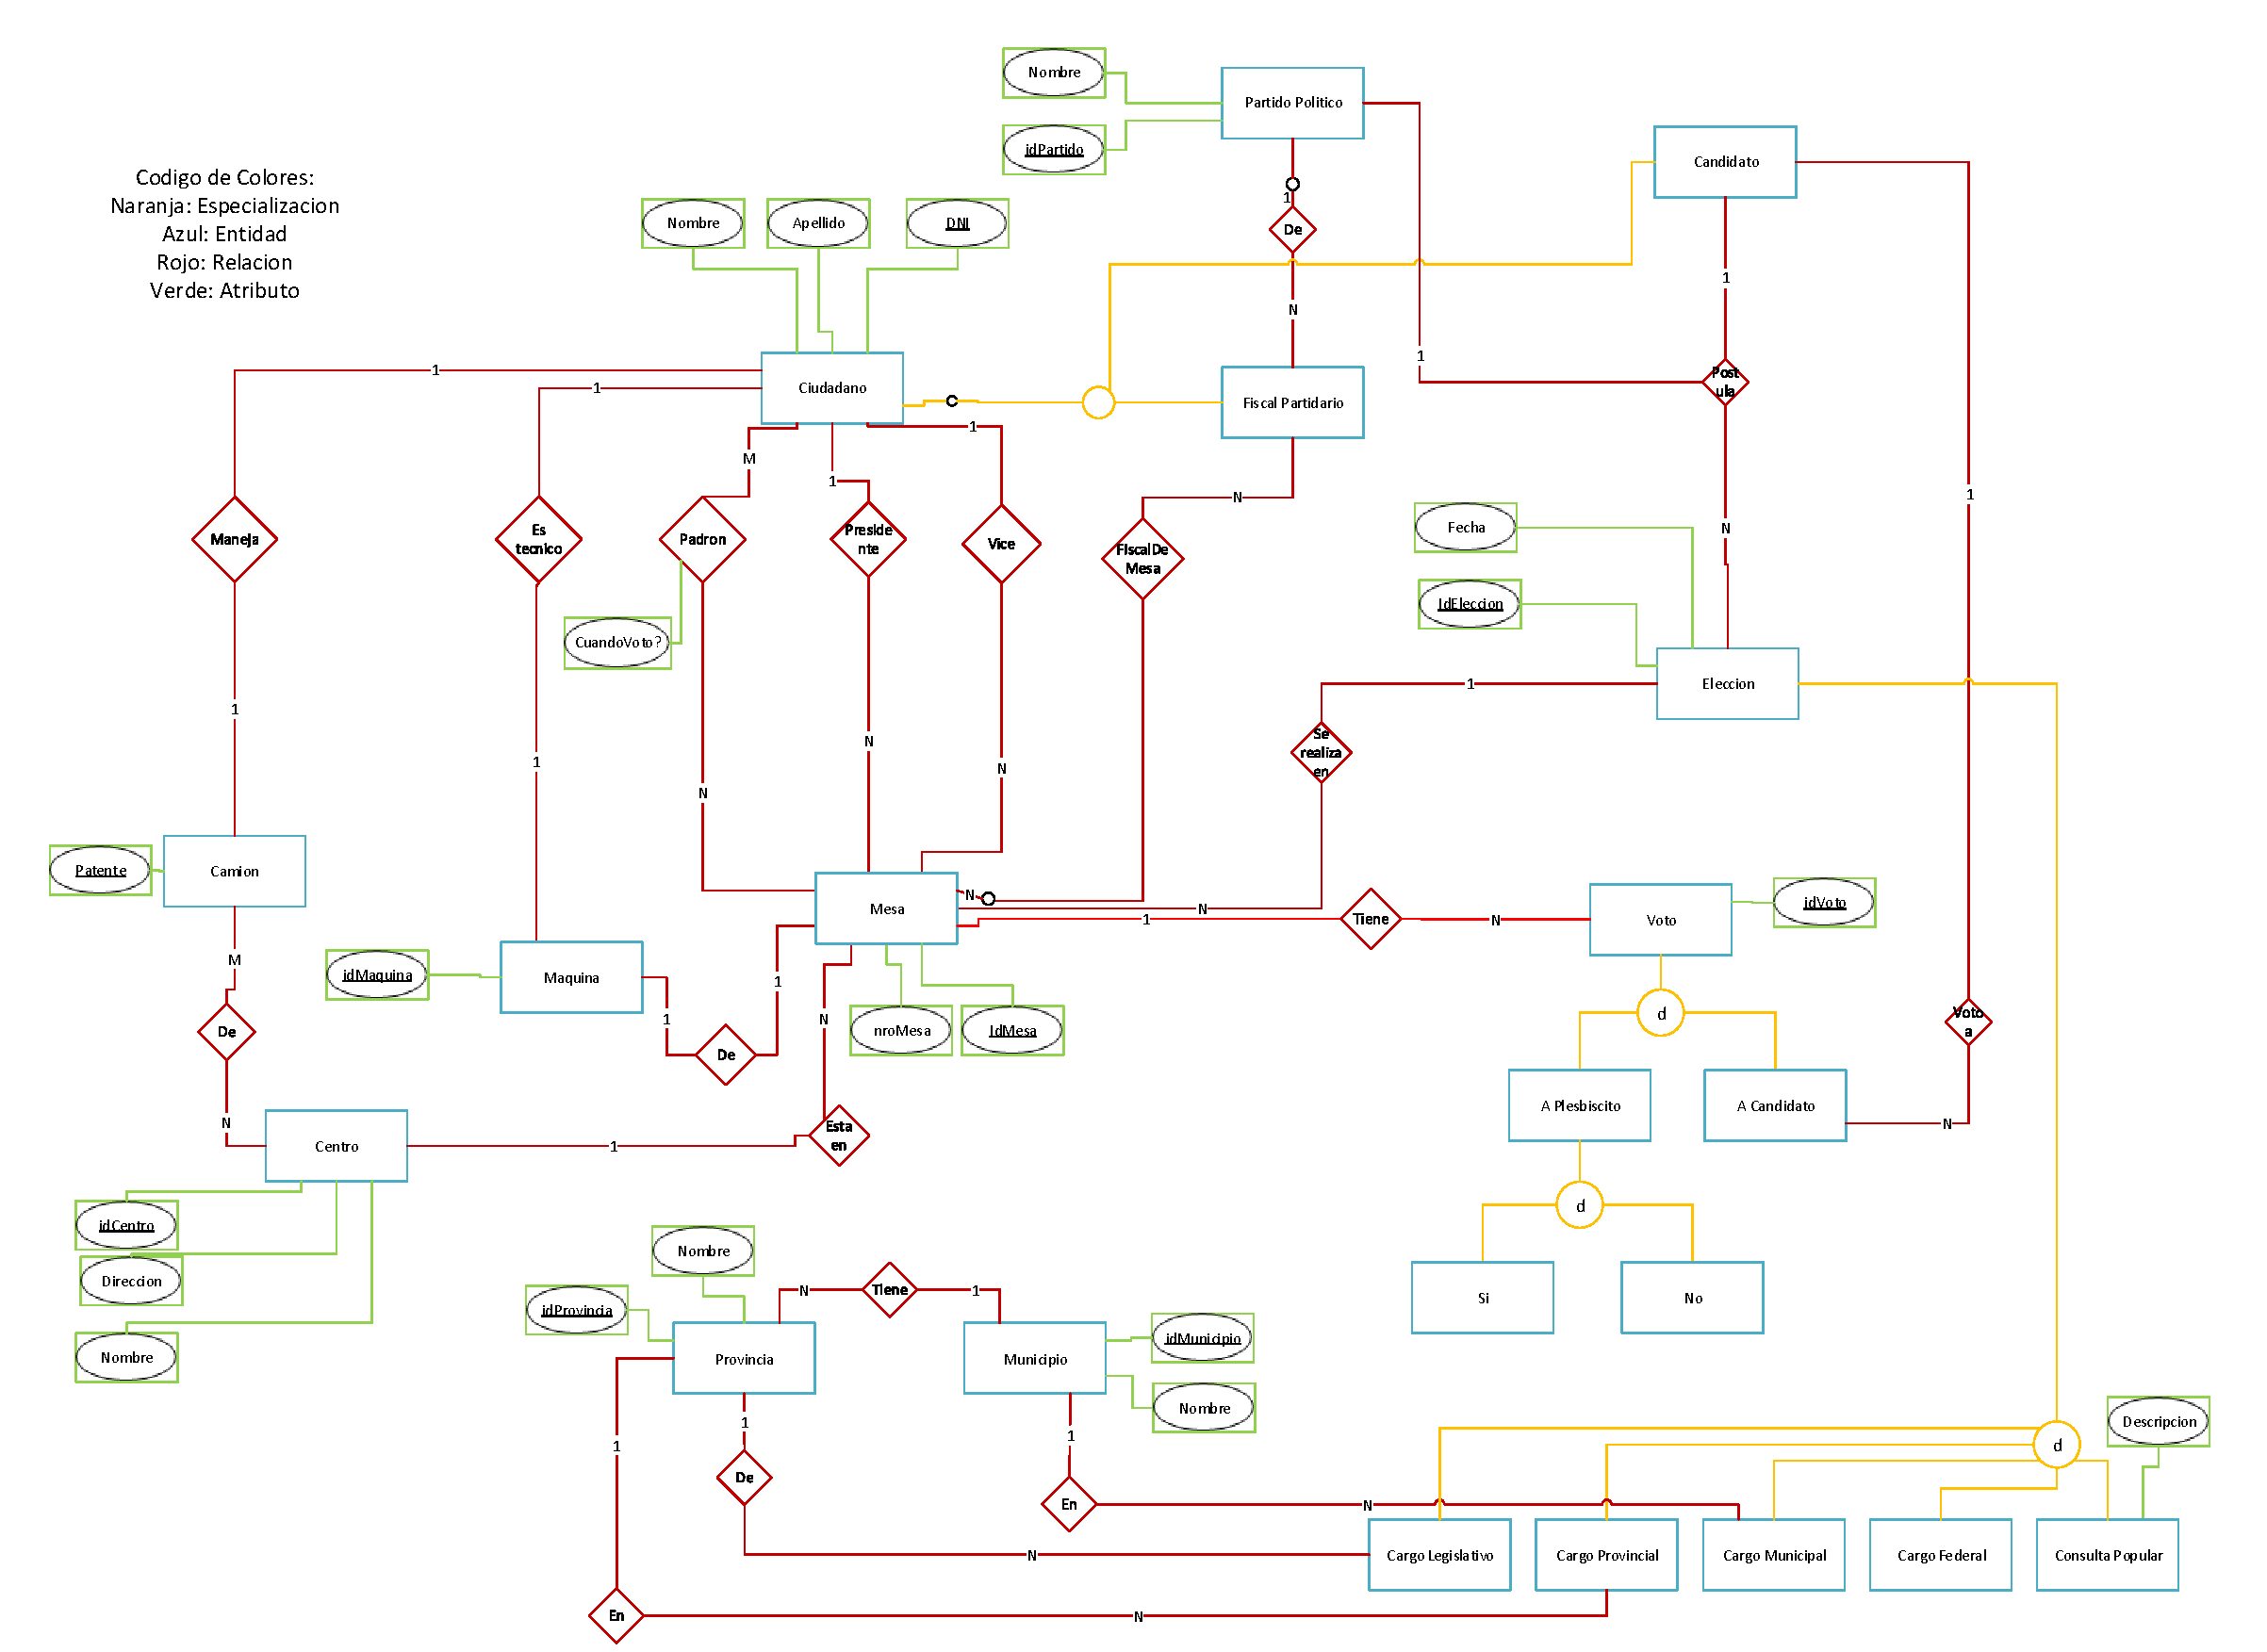
\includegraphics[scale=0.50]{fig/der.pdf}
	  \caption{Diagrama Entidad Relacion.}
	\end{figure}
\newpage

Restricciones Adicionales:

- Para cada persona que vota se debe insertar un voto(sin informacion de la persona) y actualizar correctamente la fecha y hora en la que voto y poniendo el “sello” virtual en el padron asignando un valor no nulo a cuandoVoto.

- La suma de los votos de todas las mesas de todos los candidatos debe ser menor o igual(votos en blanco diferencia) a la cantidad de ciudadanos que tiene el timestamp cuandoVoto? No nulo en el padron de dicha eleccion. (notar que esto tambien lo acota por la cantidad de ciudadanos)

- Todos los candidatos que se postulan para una eleccion, deben postularse para el mismo cargo.

- Asumimos que cada partido politico presenta un solo candidato.

- Los votos para una eleccion son: o bien consulta popular o bien de tipo candidato según corresponda el tipo de eleccion

-Si la eleccion es una consulta popular, los votos deben ser si/no. Sino, deben ser candidatos

-Un voto a candidato tiene que ser a un candidato que este postulado

- Un fiscal no puede estar en mas de una mesa en una eleccion

Habria que agregar como restriccion al der que un ciudadano no pueda ser tecnico, conductor, fiscal, etc en una misma eleccion.
\subsection{Supuestos y Restricciones}

\subsubsection{Restricciones Adicionales}

\begin{enumerate}
	\item  Para cada persona que vota se debe insertar un voto(sin informacion de la persona) y actualizar correctamente la fecha y hora en la que voto y poniendo el “sello” virtual en el padron asignando un valor no nulo a cuandoVoto.
	\item  La suma de los votos de todas las mesas de todos los candidatos debe ser menor o igual(votos en blanco diferencia) a la cantidad de ciudadanos que tiene el timestamp cuandoVoto? No nulo en el padron de dicha eleccion. (notar que esto tambien lo acota por la cantidad de ciudadanos)
	\item  Ccada partido politico presenta un solo candidato.
	\item  Todos los votos para una eleccion son: o bien consulta popular o bien de tipo candidato según corresponda el tipo de eleccion
	\item Si la eleccion es una consulta popular, los votos deben ser si/no. Sino, deben ser candidatos
	\item Un voto a candidato tiene que ser a un candidato que este postulado en esa eleccion.
	\item Un ciudadano es fiscal, presidente o vicepresidente de una sola mesa por eleccion.
	\item Un ciudadano vota en una sola mesa por eleccion.
	\item Un ciudadano no pueda ser tecnico, conductor, fiscal, etc en una misma eleccion.
\end{enumerate}

\subsection{Modelo Relacional}

\textbf{Notacion:}
\begin{itemize}
	\item \pk{Primary Key} 
	\item \fk{Not Nullable Foreign Key}
	\item \nullableFk{Nullable Foreign Key}
	\item Not Nullable Atribute
	\item \nullableAtribute{Nullable Atribute}
\end{itemize}

\vspace{2mm}
\textbf{Entidades:}
\vspace{1mm}

\begin{itemize}
	\item \textbf{Eleccion} (\pk{idEleccion}, Fecha, Tipo) 
	\begin{itemize}
		\item PK = CK = \{idEleccion\}
	\end{itemize}
	\vspace{1mm}

	\item \textbf{Eleccion\_Consulta\_Popular} (\pk{\fk{idEleccion}}, Descripcion) 
	\begin{itemize}
		\item PK = CK = FK = \{idEleccion\}
	\end{itemize}
	\vspace{1mm}

	\item \textbf{Provincia} (\pk{idProvincia}, Nombre) 
	\begin{itemize}
		\item PK = CK = \{idProvincia\}
	\end{itemize}
	\vspace{1mm}

	\item \textbf{Municipio} (\pk{idMunicipio}, Nombre, \fk{idProvincia}) 
	\begin{itemize}
		\item PK = CK = \{idMunicipio\}
		\item FK = \{idProvincia\}
	\end{itemize}
	\vspace{1mm}


	\item \textbf{Eleccion\_Cargo\_Municipal} ((\fk{\pk{idEleccion}}, \fk{idMunicipio}) 
	\begin{itemize}
		\item PK = CK = \{idEleccion\}
		\item FK = \{idEleccion, idMunicipio\}
	\end{itemize}
	\vspace{1mm}

	\item \textbf{Eleccion\_Cargo\_Provincial} ((\fk{\pk{idEleccion}}, \fk{idProvincia}) 
	\begin{itemize}
		\item PK = CK = \{idEleccion\}
		\item FK = \{idEleccion, idProvincia\}
	\end{itemize}
	\vspace{1mm}

	\item \textbf{Eleccion\_Cargo\_Legislativo} ((\fk{\pk{idEleccion}}, \fk{idProvincia}) 
	\begin{itemize}
		\item PK = CK = \{idEleccion\}
		\item FK = \{idEleccion, idProvincia\}
	\end{itemize}
	\vspace{1mm}
	 

	\item \textbf{Voto} (\pk{idVoto}, \fk{idMesa}, Tipo) 
	\begin{itemize}
		\item PK = CK = \{idVoto\}
		\item FK = \{idMesa\}
	\end{itemize}
	\vspace{1mm}

	\item \textbf{Voto\_A\_Candidato} (\pk{idVoto}, \fk{DNI}) 
	\begin{itemize}
		\item PK = CK = \{idVoto\}
		\item FK = \{idVoto, DNI (references Candidato on DNI)\}
	\end{itemize}
	\vspace{1mm}

	\item \textbf{Ciudadano} (\pk{DNI}, Nombre, Apellido, \fk{idMesa}, \nullableAtribute{selloVoto}) 
	\begin{itemize}
		\item PK = CK = \{DNI\}
		\item FK = \{idMesa\}
		\item \textbf{Nota:} selloVoto es de tipo fecha/hora, puede ser nulo y por defecto comienza siendo nulo.
	\end{itemize}
	\vspace{1mm}


	\item \textbf{Fiscal\_Partidario} (\pk{DNI}, \fk{idPartido}) 
	\begin{itemize}
		\item PK = CK = \{DNI\}
		\item FK = \{idPartido\}
	\end{itemize}
	\vspace{1mm}

	\item \textbf{Candidato} (\pk{\fk{DNI}}) 
	\begin{itemize}
		\item PK = CK = \{DNI\}
		\item FK = \{DNI references Ciudadano on DNI\}
	\end{itemize}
	\vspace{1mm}


	\item \textbf{Partido\_Politico} (\pk{idPartido}, Nombre) 
	\begin{itemize}
		\item PK = CK = \{idPartido\}
	\end{itemize}
	\vspace{1mm}

	\item \textbf{Camion} (\pk{Patente}, \fk{idConductor}) 
	\begin{itemize}
		\item PK = CK = \{Patente\}
		\item FK = \{idConductor (references Ciudadano on DNI)\}
	\end{itemize}
	\vspace{1mm}

	\item \textbf{Centro} (\pk{idCentro}, Nombre\_Establecimiento, Direccion) 
	\begin{itemize}
		\item PK = CK = \{idCentro\}
	\end{itemize}
	\vspace{1mm}

	\item \textbf{Maquina} (\pk{idMaquina}, \fk{idMesa}, \fk{idTecnico}) 
	\begin{itemize}
		\item PK = CK = \{idMaquina\}
		\item FK = \{idMesa, idTecnico (references Ciudadano on DNI)\}
	\end{itemize}
	\vspace{1mm}

	\item \textbf{Mesa} (\pk{idMesa}, nroMesa, \fk{idPresidente}, \fk{idVicepresidente}, \fk{idEleccion}, \fk{idCentro}) 
	\begin{itemize}
		\item PK = CK = \{idMesa\}
		\item FK = \{idPresidente (references Ciudadano on DNI), idVicepresidente (references Ciudadano on DNI), idEleccion, idCentro\}
	\end{itemize}
	\vspace{1mm}

\end{itemize}
		
\vspace{2mm}
\textbf{Relaciones:}
\vspace{1mm}

\begin{itemize}
	
	\item \textbf{Camion\_Centro} (\pk{\fk{patente}, \fk{idCentro}}) 
	\begin{itemize}
		\item PK = CK = \{(patente, idCentro)\}
		\item FK = \{patente, idCentro\}
	\end{itemize}
	\vspace{1mm}

	\item \textbf{Fiscales} (\pk{\fk{DNI}, \fk{idMesa}}) 
	\begin{itemize}
		\item PK = CK = \{(DNI, idMesa)\}
		\item FK = \{idMesa, DNI  (references Ciudadano on DNI)\}
		\item \textbf{Nota:} Puede haber mesas sin fiscal. Mesa participa parcialmente en esta relacion.
	\end{itemize}
	\vspace{1mm}

	\item \textbf{Postulaciones} (\pk{\fk{idEleccion}, \fk{DNI}}, \fk{idPartido}) 
	\begin{itemize}
		\item CK = \{(idEleccion, DNI), (idEleccion, idPartido)\}
		\item PK = CK = \{(idEleccion, DNI)\}
		\item FK = \{idEleccion, idPartido, DNI (references Candidato on DNI)\}
	\end{itemize}
	\vspace{1mm}

\end{itemize}

\textbf{Notas:} 
\begin{itemize}
	\item Todos los atributos en negro son no nullables.
	\item Las \pk{Primary Keys} del modelo fisico, no son autoincrement(identity) por motivos de testing.
	\item Todas las relaciones son de participacion total salvo que se explicite lo contrario.
	\item En la doble especializacion de voto por la rama de consulta popular, consideramos innecesario crear la tabla A\_Plesbicito con el campo tipo que indica si el voto es por Si o por No, pues es mas sencillo directamente especializar en el nivel superior, que un voto puede ser de 3 tipos:
	\begin{itemize}
		\item A Candidato
		\item A Consulta Popular, A favor
		\item A Consulta Popular, En contra
	\end{itemize}


\end{itemize}




\subsection{Modelo Fisico}
\subsubsection{Motor elegido}

\textbf{Microsoft Sql Server 2008}

\subsubsection{Diagrama fisico}
\subsubsection{Script de creacion de base de datos fisica}
	\begin{lstlisting}
		TODO: CREATE BBDD SCRIPT.
	\end{lstlisting}
\begin{landscape}
	\begin{figure}[t]
	  \centering	
		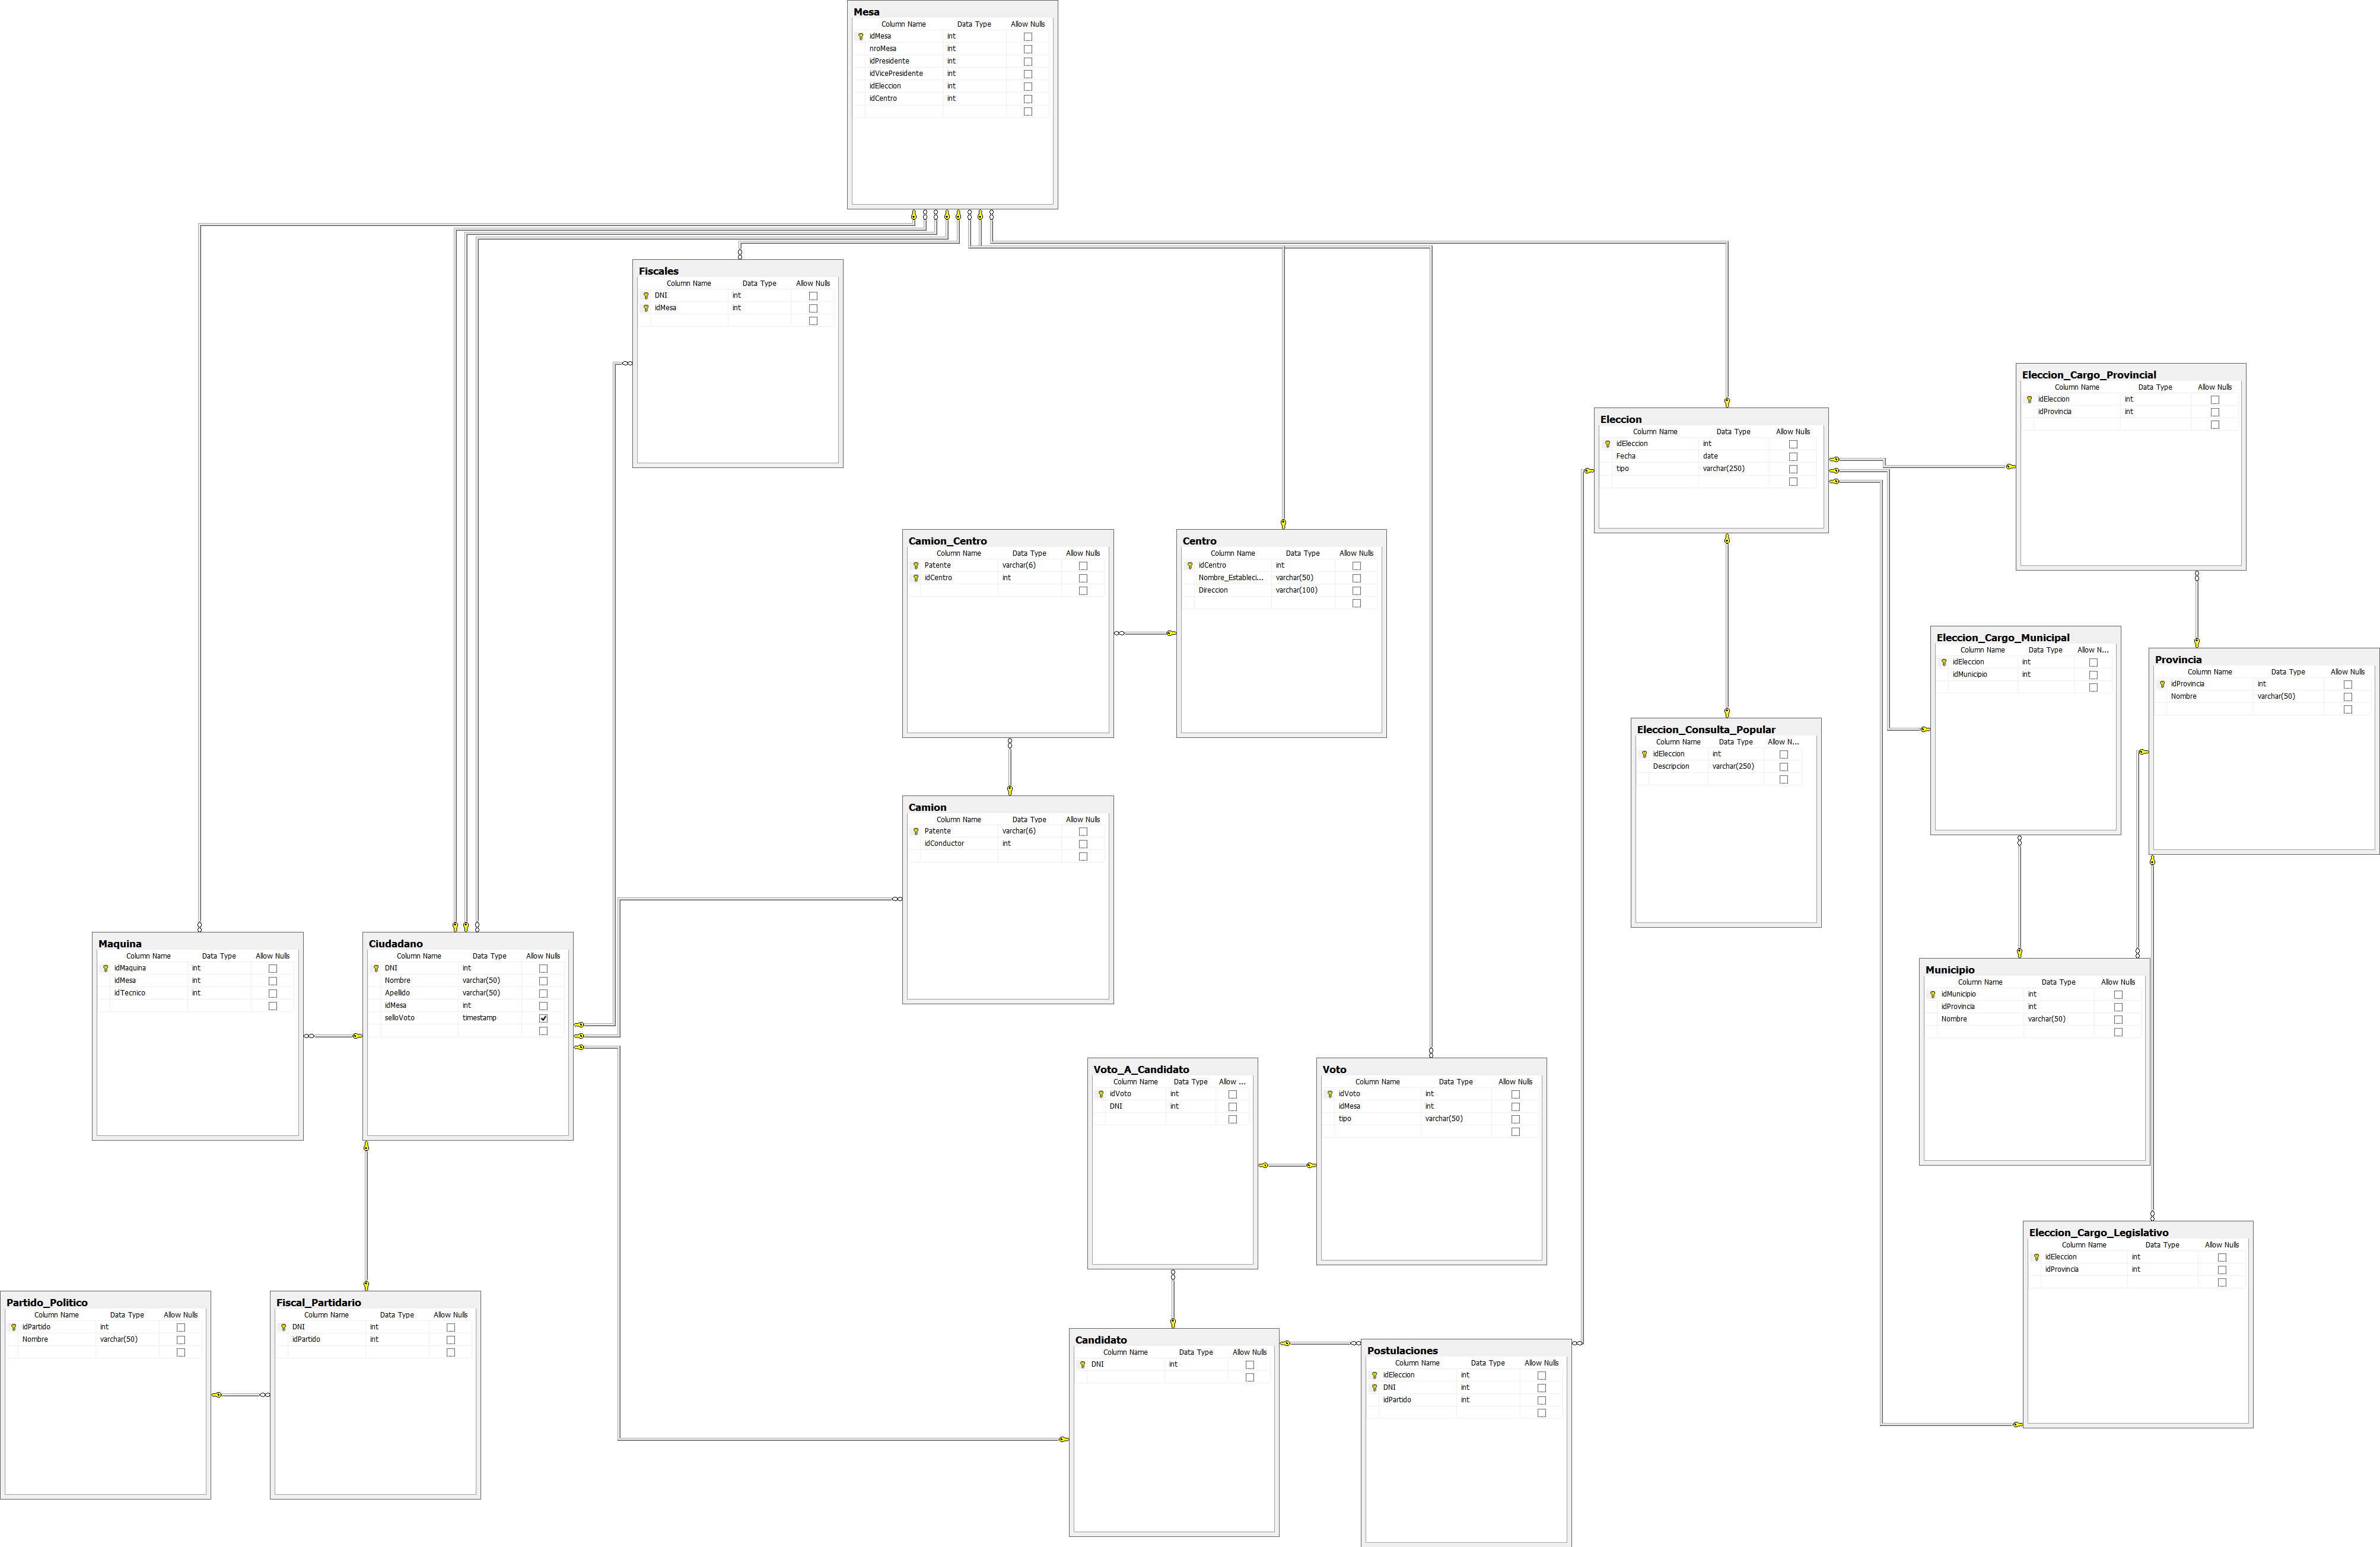
\includegraphics[scale=0.35]{fig/modelo-fisico.png}
	  \caption{Diagrama fisico.}
	\end{figure}
\end{landscape}
\subsubsection{Modelado fisico de las restricciones con triggers}
Modelaremos las restricciones al modelo utilizando funcionalidades provistas por el motor de la base de datos, como ser \textbf{Stored Procedures}, \textbf{Triggers}, \textbf{Checks}, etc. segun nos parezca conveniente. A continuacion se presenta el modelado de las restricciones.

\begin{itemize}
	\item Con respecto a las restricciones 1 y 2, referidas al voto y el sello en el padron, no podemos modelarlas con before y after triggers dado que no tenemos forma de navegar desde la tabla voto hacia el padron(no se guarda info de la persona en la tabla voto.). Con lo cual crearemos un stored procedure, que realizará la operacion de voto como una transacción, verificando que el sello sea NULO antes de insertar el voto y que el sello contenga el timestamp una vez insertado el voto. Tambien debe verificar que el voto sea a un candidato postulado para esa eleccion(la eleccion puede obtenerse de mesa), restriccion 7.
		\begin{itemize}
			\item Toda persona que vota en una mesa, debe tener nulo el campo selloVoto del padron para dicha mesa. ie. No permitir que la gente vote mas de una vez por eleccion.
			\item Para voto que se inserta se debe actualizar correctamente la fecha y hora en la que voto y poniendo el “sello” virtual en el padron asignando un valor no nulo a cuandoVoto.
			\item Un voto a candidato tiene que ser a un candidato que este postulado en esa eleccion.
		\end{itemize}

	\item Insert trigger sobre tabla voto. navegamos a mesa y de mesa a eleccion y chequeamos que el campo tipo de la eleccion corresponda con el campo tipo del voto.
		\begin{itemize}
			\item Todos los votos para una eleccion son: o bien consulta popular o bien de tipo candidato según corresponda el tipo de eleccion
			\item Si la eleccion es una consulta popular, los votos deben ser si/no. Sino, deben ser candidatos
		\end{itemize}
		\begin{lstlisting}
			CREATE TRIGGER [dbo].[trg\_check\_votoTipoEleccion] on [dbo].[Voto] AFTER INSERT AS 
			BEGIN
				SET NOCOUNT ON;
				-- Consigo el tipo de la eleccion de la mesa en la que se va a efectuar el voto
					DECLARE @tipoEleccion Varchar(250)--mismo varchar que tipo de eleccion.
					SELECT @tipoEleccion = e.tipo FROM inserted i INNER JOIN Mesa m ON m.idMesa = i.idMesa  INNER JOIN Eleccion e ON m.idEleccion = e.idEleccion
					
				-- Consigo tipo de voto a insertar
					DECLARE @tipoVoto Varchar(250)
					SELECT @tipoVoto = i.tipo FROM inserted i
					
					-- Asumo que el campo tipo esta correctamente validado en las tablas involucradas, por lo cual la eleccion puede ser a Consulta Popular o a cargos varios.
					
					IF(@tipoEleccion = 'Consulta Popular') BEGIN-- Eleccion es a consulta popular
						IF(@tipoVoto <> 'APlesbicitoSi' AND @tipoVoto <> 'APlesbicitoNo') BEGIN
							RAISERROR('La eleccion es para Consulta Popular pero el voto no es a plesbicito.', 0, 0)
							ROLLBACK TRANSACTION;
							RETURN;
						END
					END
					
					IF(@tipoEleccion <> 'Consulta Popular') BEGIN-- Eleccion es a cargo
						IF(@tipoVoto <> 'ACandidato') BEGIN
							RAISERROR('La eleccion es para Cargo pero el voto no es a candidato.', 0, 0)
							ROLLBACK TRANSACTION;
							RETURN;
						END
					END
			END;
		\end{lstlisting}
	
	\item{Queda implicada por el stored procedure de voto, que chequea sello null y marca no null el sello luego. No hay forma que de se inserten mas votos que personas}. \fk{Alguien piense esto a ver si no estoy flasheando plz.}
		\begin{itemize}
			\item La suma de los votos de todas las mesas de todos los candidatos debe ser menor o igual(votos en blanco diferencia) a la cantidad de ciudadanos que tiene el timestamp cuandoVoto? No nulo en el padron de dicha eleccion. (notar que esto tambien lo acota por la cantidad de ciudadanos). 
		\end{itemize}

	\item Queda determinado por la PK de la tabla Postulaciones.
		\begin{itemize}
			\item No hay candidatos repetidos en una eleccion.
		\end{itemize}

	\item Insert trigger en postulaciones que no permita hacer insert si ya existe un candidato para dicho partido politico en dicha eleccion.
		\begin{itemize}
			\item Cada partido politico presenta un solo candidato.
		\end{itemize}
		\begin{lstlisting}
			CREATE TRIGGER trg_check_selloVotoEsNull on Postulaciones INSTEAD OF INSERT AS 
			BEGIN
				SET NOCOUNT ON
					INSERT INTO Postulaciones(
						SELECT * FROM INSERTED
						WHERE 
						)
					blablabla, TODO
			END
		\end{lstlisting}
	
	\item Insert trigger en Mesa que verifique que en esa eleccion, no haya otras mesas donde este ciudadano sea tecnico, presidente, vicepresidente, fiscal o conductor. \textbf{Esto debe incluir que en la mesa a insertar este el mismo DNI en varias FK.}
	\item Insert trigger en Conductor que verifique que en esa eleccion, no haya  mesas donde este ciudadano sea tecnico, presidente, vicepresidente o fiscal.
		\begin{itemize}
			\item Un ciudadano no pueda ser tecnico, presidente, vicepresidente o fiscal en una misma eleccion.
			\item Un ciudadano no puede ser conductor y tecnico, presidente, vicepresidente o fiscal en una misma eleccion.
		\end{itemize}	

	\item Insert trigger en Padron que verifique que para ese DNI, no exista otra mesa, de la misma eleccion, que ya lo tenga asociado.
		\begin{itemize}
			\item Un ciudadano vota en una sola mesa por eleccion.
		\end{itemize}

	\item Insert en Mesa para ver que la maquina asignada no este asignada a otra mesa en esa eleccion.
		\begin{itemize}
			\item Una maquina funciona en una sola mesa por eleccion.
		\end{itemize}

\end{itemize}



\fk{Hay que hacer triggers para validar los campos tipo de las tablas que tengan herencia. O ver si hay alguna forma de especificar tipos enumerados en SQLSERVER2008}

\fk{OJO QUE VAMOS A USAR TRANSACCION EN UN STORED PROCEDURE.}
ojo con los insert triggers y los updates, habria que prohibir los updates o hacer triggers en insert y update?
no se deberian permitir deletes ni updates sobre voto(y posiblemente otras tablas). ??


--Utiles para testear triggers rapido
--ALTER TABLE Voto NOCHECK CONSTRAINT ALL
--ALTER TABLE Voto CHECK CONSTRAINT ALL
\subsection{Codigo de resolucion de consignas}
\subsubsection{Script de creacion de base de datos fisica}
Por motivos de latex y caracteres, no se pueden incluir los scripts. Los scripts .sql se encuentran en la carpeta fuentes.

\subsubsection{Consultas pedidas por el enunciado}
\begin{enumerate}
	\item Poder obtener los ganadores de las elecciones transcurridas en el último año.
		Para resolver este problema nos creamos una vista auxiliar que nos devuelve la lista de elcciones del ultimo a\~no, 
		con sus resultados, es decir, el ranking (Candidato, CantVotos) para cada eleccion del último año.

		\begin{lstlisting}
		CREATE VIEW [dbo].[Ranking_Elecciones_Cargo_Ultimo_Anio] AS
		--Vista auxiliar para ranking de las ultimas elecciones del anio.
		SELECT 
	elec.Fecha as FechaEleccion, 
	elec.tipo as TipoEleccion,
	(ciu.Nombre + ciu.Apellido) as Candidato, 
	COUNT(vc.idVoto) AS CantVotos
FROM         dbo.Voto AS v 
INNER JOIN dbo.Voto_A_Candidato AS vc ON v.idVoto = vc.idVoto -- Quiero saber a que candidato fue ese voto
INNER JOIN dbo.Ciudadano AS ciu ON vc.DNI= ciu.DNI -- Join para saber el nombre del candidato(es un ciudadano)
INNER JOIN dbo.Mesa AS m ON m.idMesa = v.idMesa -- Join para saber la eleccion de la mesa y agrupar
INNER JOIN dbo.Eleccion AS elec ON elec.idEleccion = m.idEleccion -- Join para saber la fecha de la eleccion
WHERE	(v.idMesa IN
	(SELECT     idMesa
	FROM          dbo.Mesa AS m
	WHERE      (idEleccion IN
		(SELECT     idEleccion
		FROM          dbo.Eleccion AS e
		WHERE      (YEAR(Fecha) = YEAR(GETDATE()))))))
GROUP BY vc.DNI, ciu.Nombre, ciu.Apellido, elec.Fecha, elec.tipo
ORDER BY FechaEleccion ASC, CantVotos DESC

		\end{lstlisting}
		
	Luego aplicamos una consulta sobre esta vista, que nos devuelve para cada eleccion de la vista, el (o los en caso de empate) ganador(es).
	Creamos otra vista para acceder directamente a esta consulta pedida.
		
		\begin{lstlisting}
			CREATE VIEW [dbo].[Ganadores_Elecciones_Cargo_Ultimo_Anio] AS
			SELECT FechaEleccion, Candidato, MAX(CantVotos) as ganador_con_max_votos
			FROM Ranking_Elecciones_Cargo_Ultimo_Anio
			GROUP BY FechaEleccion, Candidato
		\end{lstlisting}

		Finalmente, se accede a los datos pedidos ejecutando:
		\begin{lstlisting}
			SELECT * FROM dbo.[Ganadores_Elecciones_Cargo_Ultimo_Anio]
		\end{lstlisting}

	\item Poder consultar las cinco personas que más tarde fueron a votar antes de terminar
	la votación por cada centro electoral en una elección.
	Usamos una tabla intermedia que obtiene los votos de la eleccion, particionado por centro electoral, a su vez, utilizamos la funcion \texttt{ROW\_NUMBER} para numerar los resultados de cada grupo, ordenados por tiempo de votacion y quedarnos con los 5 mayores tiempos de votacion de cada centro.
	\begin{lstlisting}
		WITH TOPFIVE AS (
	    SELECT cen.Nombre_Establecimiento, (ciu.Nombre + ciu.Apellido) as Votante, p.selloVoto as HoraVoto,
	    ROW_NUMBER() over (
	        PARTITION BY cen.idCentro
	        ORDER BY p.selloVoto DESC
	    ) AS NumFila
	    FROM Padron p
	    INNER JOIN Mesa m ON m.idMesa = p.idMesa
	    INNER JOIN Centro cen ON cen.idCentro = m.idCentro
	    INNER JOIN Ciudadano ciu ON ciu.DNI = p.DNI
	    
	SELECT Nombre_Establecimiento, Votante, HoraVoto FROM TOPFIVE WHERE NumFila <= 5--cantidad de items por grupo
	\end{lstlisting}

	\item Poder consultar quienes fueron los partidos políticos que obtuvieron más del 20\%
	en las últimas cinco elecciones provinciales a gobernador.
	\textbf{Nota:} En las elecciones a cargo provincial se elije gobernador(legislativas y municipales estan separadas de las provinciales).\\

Creamos una vista que nos devuelve el ranking de las ultimas 5 elecciones a gobernador, y ademas la cantidad de votos por cada eleccion.

\begin{lstlisting}
	SELECT elec.Fecha AS FechaEleccion, ciu.Nombre + ciu.Apellido AS Candidato, partPolitico.Nombre as PartidoPolitico, 
COUNT(vc.idVoto) AS CantVotos,  

COUNT(*) over (
	        PARTITION BY elec.fecha
	    ) AS Cant_Total_Votos_Por_Eleccion  

FROM         dbo.Voto AS v 
                      INNER JOIN dbo.Voto_A_Candidato AS vc ON v.idVoto = vc.idVoto 
                      INNER JOIN dbo.Ciudadano AS ciu ON vc.DNI = ciu.DNI 
                      INNER JOIN dbo.Mesa AS m ON m.idMesa = v.idMesa 
                      INNER JOIN dbo.Eleccion AS elec ON elec.idEleccion = m.idEleccion
                      INNER JOIN dbo.Postulaciones post ON (post.idEleccion = elec.idEleccion AND post.DNI = ciu.DNI)
                      INNER JOIN dbo.Partido_Politico partPolitico ON post.idPartido = partPolitico.idPartido
WHERE     (v.idMesa IN
              (SELECT     idMesa
                FROM          dbo.Mesa AS m
                WHERE      (idEleccion IN
		           (SELECT     TOP (5) e.idEleccion
		             FROM          dbo.Eleccion AS e INNER JOIN
		                                    dbo.Eleccion_Cargo_Provincial AS ecp ON ecp.idEleccion = e.idEleccion
		             WHERE      (e.tipo = 'Cargo Provincial') AND (YEAR(e.Fecha) = YEAR(GETDATE()))
		             ORDER BY e.Fecha DESC))))
GROUP BY vc.DNI, partPolitico.Nombre, ciu.Nombre, ciu.Apellido, elec.Fecha
\end{lstlisting}

Creamos otra vista que sobre la vista anterior, calcula el porcentaje de votos de cada partido y lo filtra por quienes tienen mas de 20\%.

\begin{lstlisting}
SELECT     TOP (100) PERCENT FechaEleccion, PartidoPolitico, CantVotos * 100 / Cant_Total_Votos_Por_Eleccion AS Porcentaje
FROM         dbo.Ranking_Candidatos_Ultimas_5_Elecciones_A_Gobernador
WHERE     (CantVotos * 100 / Cant_Total_Votos_Por_Eleccion >= 20)
ORDER BY FechaEleccion, CantVotos DESC
\end{lstlisting}

Finalmente, consultamos la vista.

\begin{lstlisting}
	SELECT * FROM Partidos_Con_Mas_Del_20_Porciento_Ultimas_5_Gobernador
\end{lstlisting}

\end{enumerate}
\subsection{Codigo de testing de la solucion provista}

En primera instancia, se realizaran pruebas de solidez y correctitud de las restricciones implementadas. Por último, tests de correctitud de las consultas requeridas por el enunciado. El codigo de los tests de restricciones se encuentra en 'tests.sql'

\subsubsection{Votos de una eleccion}

Verificaremos la conjuncion de las restricciones "Todos los votos para una eleccion son: o bien consulta popular o bien de tipo candidato según corresponda el tipo de eleccion",  "Si la eleccion es una consulta popular, los votos deben ser si/no. sino, deben ser candidatos'' y por ultimo, ''Un voto a candidato, debe referenciar a un candidato postulado para dicha eleccion''

\begin{enumerate}

\item \textbf{Consulta Popular:} Si la eleccion es una consulta popular, los votos cuya clave foranea
referencia esa eleccion deben ser de tipo ' A Plesbiscito Si ' o ' A Plesbiscito No'. Creamos una elección de tipo 'Consulta Popular' utilizando la Stored Procedure 'Crear\_ Consulta\_ Popular' con los valores Descripcion: TEST y Fecha: '2015-06-09'. 

A continuacion, debemos crear una mesa. Para eso, debemos tener un presidente, un vicepresidente,
un centro y una maquina(y para ella, un tecnico). Las creamos ejecutando:

\begin{lstlisting}

INSERT INTO Ciudadano VALUES
 (1,'JUAN','VOTANTE'),
 (2,'PEPE','PRESIDENTE'),
 (3,'VICTOR','VICEPRESIDENTE'),
 (4,'TOMAS','TECNICO'),
 
 INSERT INTO Centro VALUES
 (1,'Escuela', '9 de julio 1');

 INSERT INTO Maquina VALUES
 (1,4);

 INSERT INTO Mesa VALUES
 (1,1,2,3,1,1,1);
\end{lstlisting}

	\begin{itemize}
	\item 'A Plesbiscito Si': Insertar un voto 'A Plesbiscito Si' deberia realizarse correctamente. (En todos los casos, al terminar el test borramos el voto)
	Ejecutamos la Stored Procedure 'Votar\_ Consulta\_ Popular' con los parametros DNIdelVotante=1, idEleccion=1 y OpcionVoto=1. Acto seguido, ejecutamos:
	\begin{lstlisting}
	SELECT * FROM Voto
	\end{lstlisting}
	Y efectivamente esto nos da como resultado:	
	\vspace{2mm}
	
	\begin{tabular}{| l| l| l| l| }
	\hline 
	   & idVoto & idMesa & Tipo \\
	   \hline
	 1 & 1 & 1 & A Plesbiscito Si \\
 	 \hline 
	\end{tabular}
	
	\vspace{2mm}
	\item 'A Plesbiscito No': Insertamos un voto de tipo 'A Plesbiscito No', lo cual deberia ejecutarse correctamente, usando la Stored Procedure 'Votar\_ Consulta\_ Popular' con los parametros DNIdelVotante=1, idEleccion=1 y OpcionVoto=0. Resultado:
	
	\begin{tabular}{| l| l| l| l| }
	\hline 
	   & idVoto & idMesa & Tipo \\
	   \hline
	 1 & 1 & 1 & A Plesbiscito No \\
 	 \hline 
	\end{tabular}
	
	\vspace{2mm}	
	
	\item 'Voto de tipo invalido': Insertamos un voto de tipo invalido, lo cual NO deberia ejecutarse correctamente, usando la Stored Procedure 'Votar\_ Consulta\_ Popular' con los parametros DNIdelVotante=1, idEleccion=1 y OpcionVoto=3 (Esto representa un tipo de voto invalido). Resultado:
	
\begin{tabular}{| l| l| l| l| }
	\hline 
	   & idVoto & idMesa & Tipo \\
	   \hline
	 &  &  &  \\
 	 \hline 
	\end{tabular}
	
	\vspace{2mm}	
		
	
	\item 'Voto a un candidato': Insertamos un voto 'A Candidato' lo cual NO deberia ejecutarse correctamente, usando la Stored Procedure 'Votar\_ Candidato' sobre la Consulta Popular, con los parametros DNIdelVotante=1, idEleccion=1 y DniCandidato=5. Inmediatamente recibimos el aviso:
	''La eleccion es para Consulta Popular pero el voto no es a plesbicito''. y como resultado:
		
\begin{tabular}{| l| l| l| l| }
	\hline 
	   & idVoto & idMesa & Tipo \\
	   \hline
	 &  &  &  \\
 	 \hline 
	\end{tabular}
	
	\vspace{2mm}	
	\end{itemize}
\item \textbf{Eleccion a candidato:}  Si la eleccion es de tipo 'Cargo Federal', 'Cargo Municipal', Cargo Provincial' o tipo 'Cargo Legislativo', los votos cuya clave foranea referencia esa eleccion deben ser de tipo 'A Candidato', y deben referenciar a un candidato que este postulado a dicha eleccion. Vamos a crear una eleccion provincial, debemos crear una provincia, un partido, y postular a 'CARLOS CANDIDATO' a la eleccion.
\begin{lstlisting}
	 INSERT INTO Ciudadano VALUES
	(5,'CARLOS', 'CANDIDATO');
 
  	INSERT INTO Candidato VALUES
 	(5);

	INSERT INTO Provincia VALUES
 	(1,'BUENOS AIRES');
 	 
 	INSERT INTO Partido_Politico VALUES
	(1,'FRENTE POR LA APROBACION');
	
	INSERT INTO Postulaciones VALUES
	(1,5,1)
	\end{lstlisting}
	
Eliminamos la anterior eleccion, de forma de poder usar la misma mesa y sus encargados, y usamos la Stored Procedure 'Crear\_ Eleccion\_ Provincial', con los parametros idProvincia=1 y fecha='2015-06-10'.

	\begin{itemize}
	\item 'Candidato Valido': Insertamos un voto de tipo 'A candidato', cuya clave foranea a candidato referencia a un candidato cuyo DNI se encuentra en la tabla postulaciones para esa eleccion, lo cual deberia ejecutarse sin problemas. Usamos la Stored Procedure: 'Votar\_ Candidato' con los parametros: DNIVotante=1, idEleccion=1, DNICandidato=5.Si ejecutamos:
	\begin{lstlisting}
	SELECT * FROM Voto
	\end{lstlisting}
	
	Obtenemos:
	
	\begin{tabular}{| l| l| l| l| }
	\hline 
	   & idVoto & idMesa & Tipo \\
	   \hline
	 1 & 1 & 1 & A Candidato \\
 	 \hline 
	\end{tabular}
	\vspace{2mm}	
	
	Y si ejecutamos: 
	
	\begin{lstlisting}
	SELECT * FROM Voto_A_Candidato
	\end{lstlisting}
	
	Obtenemos:
	
	\begin{tabular}{| l| l|}
	\hline 
	   idVoto & DNI \\
	   \hline
	 1 & 5  \\
 	 \hline 
	\end{tabular}
	\vspace{2mm}
	
	\item 'Candidato Invalido': e insertamos un voto de tipo 'A candidato', cuya clave foranea a candidato NO referencia a un candidato cuyo DNI se encuentra en la tabla postulaciones para esa eleccion. Esto no deberia ser aceptable. Para esto creamos otro ciudadano:
	\begin{lstlisting}
	 INSERT INTO Ciudadano VALUES
 	(6,'IGNACIO','IMPOSTOR');
	\end{lstlisting}
	
	Usamos la Stored Procedure: 'Votar\_ Candidato' con los parametros: DNIVotante=1, idEleccion=1, DNICandidato=6. Obtenemos un aviso: 'Instrucción INSERT en conflicto con la restricción FOREIGN KEY "FK\_Voto\_ A\_ Candidato\_ Candidato'. Y los resultados de consultar la tabla Voto y la tabla Voto\_ A\_ Candidato son:
	
	
	\begin{tabular}{| l| l| l| l| }
	\hline 
	   & idVoto & idMesa & Tipo \\
	  \hline 
	   & & & \\
	   \hline 
	\end{tabular}
	\vspace{2mm}	
	
	
	\begin{tabular}{| l| l|}
	\hline 
	idVoto & DNI \\
	\hline 
	 & \\
	\hline 
	\end{tabular}
		
	\item 'Voto a plesbiscito': Insertamos un voto
	de tipo 'A plesbiscito Si', lo cual no deberia ejecutarse. Ejecutamos la Stored Procedure 'Votar\_ Consulta\_ Popular' con los parametros DNIdelVotante=1, idEleccion=1 y OpcionVoto=1. Obtenemos el aviso: ''La eleccion es para Cargo pero el voto no es a candidato'', y como resultados:
	
	\begin{tabular}{| l| l| l| l| }
	\hline 
	   & idVoto & idMesa & Tipo \\
	  \hline 
	   & & & \\
	   \hline 
	\end{tabular}
	\vspace{2mm}	
	
	
	\begin{tabular}{| l| l|}
	\hline 
	idVoto & DNI \\
	\hline 
	 & \\
	\hline 
	\end{tabular}
			
	\end{itemize}
\end{enumerate}
\subsubsection{Multiples Candidatos:} Un partido politico puede presentar a un solo candidato por eleccion. Para chequear esto, vamos a intentar postular a ambos 'CARLOS CANDIDATO' e 'IGNACIO IMPOSTOR' al partido 'Frente por la Aprobacion'. No deberia ejecutarse. Al ejecutar esto, obtenemos el aviso: ''Infracción de la restricción UNIQUE KEY 'Unique\_ Key\_ Eleccion\_ Partido''. Si consultamos la tabla postulaciones, nos devuelve:
\vspace{2mm}
	
	\begin{tabular}{| l| l| l|}
	\hline 
	idEleccion & DNI & idPartido \\
	\hline 
	 1 & 5 & 1 \\
	\hline 
	\end{tabular}
\vspace{2mm}
Con lo que efectivamente, no se inserto el segundo candidato.

\subsubsection{Multiples Mesas para un ciudadano:} Un ciudadano solo vota en una mesa por eleccion. Para comprobar eso creamos otro presidente, vicepresidente, tecnico y maquina para poder crear otra mesa, e intentamos asignar en el Padron a 'PEPE VOTANTE' ambas mesas.
	\begin{lstlisting}
	INSERT INTO Ciudadano VALUES
	(7,'TITO','TECNICODOS'),
	(8,'PEDRO','PRESIDENTEDOS'),
	(9,'VALENTIN','VICEPRESIDENTEDOS');
	
	INSERT INTO Maquina VALUES
 	(2,7);
 	
 	 INSERT INTO Mesa VALUES
 	(2,2,8,9,1,1,2)
 
	\end{lstlisting}
	\vspace{2mm}		
	Y finalmente, asignamos al ciudadano a ambas mesas
	\vspace{2mm}
	\begin{lstlisting}
	Insert INTO Padron VALUES
	(1,1,NULL)
	(1,2,NULL)
	\end{lstlisting}
	
	\vspace{2mm}
	
	A lo que recibimos el aviso: ''Ya existe una mesa en la cual esta persona vota en esta eleccion''. Y si consultamos el padron, obtenemos:
	
	\vspace{2mm}
	
	\begin{tabular}{| l| l| l|}
	\hline 
	DNI & idMesa & selloVoto \\
	\hline 
	 1 & 1 & NULL \\
	\hline 
	\end{tabular}
	\vspace{2mm}
	
	Efectivamente solo se asigno la primera vez.
	
\subsubsection{Multiples Mesas para una  maquina:} Una maquina solo funciona en una mesa por eleccion. Para esto eliminamos la segunda mesa que creamos en el test anterior, y la vamos a crear de nuevo pero asignandole la misma maquina 1.
	\begin{lstlisting}
	 DELETE FROM Mesa 
 	 WHERE idMesa=2
 	 
 	 
 INSERT INTO Mesa VALUES
 	  (2,2,8,9,1,1,1);
	\end{lstlisting}
			\vspace{2mm}				
Obtenemos el aviso: ''Ya existe una mesa en esta eleccion con esta maquina'', y si consultamos la tabla Mesa vemos que efectivamente no se agrego la segunda:
			\vspace{2mm}	
			
	\begin{tabular}{| l| l| l| l| l| l| l|}
	\hline 
	idMesa & nroMesa & idPresidente & idVicePresidente & idEleccion & idCentro & idMaquina \\
	\hline 
	 1 & 1 & 2 & 3 & 1 & 1 & 1 \\
	\hline 
	\end{tabular}
	
	\vspace{2mm}	
			
\subsubsection{Validaciones de los votos}: Validaremos las restricciones: ''No permitir que la gente vote mas de una vez por eleccion'', ''El voto puede hacerse en la fecha de la eleccion de 8am a 6pm''. 
	\begin{itemize}
	\item 'Unico voto': Creamos un partido politico para el Candidato 'IGNACIO IMPOSTOR' y lo postulamos

	\begin{lstlisting}
	INSERT INTO Partido_Politico VALUES
	(2,'UNIDOS POR LA UNION');
	
	
	INSERT INTO Postulaciones VALUES
	(1,5,1);
	(1,6,2);
	\end{lstlisting}

 Usamos dos veces consecutivas la Stored Procedure: 'Votar\_ Candidato' con los parametros: DNIVotante=1, idEleccion=1, DNICandidato=5 en la primera vez, y en la segunda vez: DNIVotante=1, idEleccion=1, DNICandidato=6. Obtenemos el aviso: 'Esta persona ya voto en esta eleccion', y como resultado:
 
 	\vspace{2mm}	
 	
 \begin{tabular}{| l| l| l| l| }
	\hline 
	   & idVoto & idMesa & Tipo \\
	  \hline 
	   &1 &1 & aCandidato \\
	   \hline 
	\end{tabular}
	\vspace{2mm}	
	
		\vspace{2mm}
			
	\begin{tabular}{| l| l|}
	\hline 
	idVoto & DNI \\
	\hline 
	  1 & 5 \\
	\hline 
	\end{tabular}
	
		\vspace{2mm}	
		Donde vemos que solo se inserto el primer voto.
		
	\item 'Hora valida': Creamos una elección de tipo 'Consulta Popular', y hacemos que un ciudadano intente votar en un horario invalido (cambiamos la hora de la computadora a las 19:00hs). Recibimos el aviso:Estamos fuera de horario de votacion, y no se modificaron las tablas de votos.

	
	\end{itemize}					

\subsubsection{Consultas del enunciado}:

Insertamos los siguientes datos en la base para poder realizar los dos primeros tests: 15 ciudadanos, que seran los votantes, dos presidentes, vicepresidentes y tecnicos de mesa, dos candidatos, dos conductores(a estos ultimos, no los hacemos votar, solo hacemos votar a los ciudadanos para que sea mas entendible), dos centros, dos camiones, una provincia y dos partidos. Este codigo se encuentra en el archivo 'testQueries.sql'

\begin{lstlisting}
INSERT INTO Ciudadano VALUES
(1,'CIUDADANO','UNO'),
(2,'CIUDADANO','DOS'),
(3,'CIUDADANO','TRES'),
(4,'CIUDADANO','CUATRO'),
(5,'CIUDADANO','CINCO'),
(6,'CIUDADANO','SEIS'),
(7,'CIUDADANO','SIETE'),
(8,'CIUDADANO','OCHO'),
(9,'CIUDADANO','NUEVE'),
(10,'CIUDADANO','DIEZ'),
(11,'CIUDADANO','ONCE'),
(12,'CIUDADANO','DOCE'),
(13,'CIUDADANO','TRECE'),
(14,'CIUDADANO','CATORCE'),
(15,'CIUDADANO','QUINCE'),
(16,'PRESIDENTEMESA','UNO'),
(17,'PRESIDENTEMESA','DOS'),
(18,'VICEPRESIDENTEMESA','UNO'),
(19,'VICEPRESIDENTEMESA','DOS'),
(20,'TECNICO','UNO'),
(21,'TECNICO','DOS'),
(22,'CANDIDATO','UNO'),
(23,'CANDIDATO','DOS'),
(24,'CANDIDATO','TRES'),
(25,'CANDIDATO','CUATRO'),
(26,'CONDUCTOR','UNO'),
(27,'CONDUCTOR','DOS');

INSERT INTO Centro VALUES
(1,'ESCUELA','UNO'),
(2,'ESCUELA2','DOS');

INSERT INTO Camion VALUES
(1,26),
(2,27);

INSERT INTO Camion_Centro VALUES
(1,1),
(2,2);

INSERT INTO Maquina VALUES
(1,20),
(2,21);

INSERT INTO Candidato VALUES
(22), (23), (24), (25);

INSERT INTO Provincia VALUES
(1,'BUENOS AIRES');

INSERT INTO Partido_Politico VALUES
(1,'PARTIDO DE IZQUIERDA'),
(2,'PARTIDO DE DERECHA');


\end{lstlisting}

\begin{itemize}
\item \textbf{Ganadores de elecciones del ultimo año}
A continuacion creamos dos elecciones, una federal y una provincial. Cambiamos el reloj de la computadora al 1 de enero de 2015 para crear la federal, para poder estar la correctitud del calculo del año corriente, y la provincial se efectua el 12/06/2015. Usamos la Stored Procedure para crear la provincial, y el siguiente codigo para crear la federal:

\begin{lstlisting}
INSERT INTO Eleccion VALUES
(1,GETDATE(),'Cargo Federal');
\end{lstlisting}


A continuacion creamos dos mesas, una en cada centro y para cada eleccion. Acto seguido, postulamos a los primeros dos candidatos a la eleccion del 1ero de enero, uno por el partido de izquierda, el otro por el de derecha. Hacemos lo mismo con el tercer y cuarto candidato, en la eleccion del 12 de junio.

\begin{lstlisting}
INSERT INTO Mesa VALUES
(1,1,16,18,1,1,1);

INSERT INTO Mesa VALUES
(2,2,17,19,2,2,2);

INSERT INTO Postulaciones VALUES
(1,22,1),
(1,23,2),
(2,24,1),
(2,25,2);
\end{lstlisting}

Finalmente, armamos el padron y asignamos a los 15 ciudadanos, la mesa 1 para la primera eleccion y la mesa 2 para la segunda eleccion.

\begin{lstlisting}
INSERT INTO Padron VALUES
(1,1,NULL),
(2,1,NULL),
(3,1,NULL),
(4,1,NULL),
(5,1,NULL),
(6,1,NULL),
(7,1,NULL),
(8,1,NULL),
(9,1,NULL),
(10,1,NULL),
(11,1,NULL),
(12,1,NULL),
(13,1,NULL),
(14,1,NULL),
(15,1,NULL),
(1,2,NULL),
(2,2,NULL),
(3,2,NULL),
(4,2,NULL),
(5,2,NULL),
(6,2,NULL),
(7,2,NULL),
(8,2,NULL),
(9,2,NULL),
(10,2,NULL),
(11,2,NULL),
(12,2,NULL),
(13,2,NULL),
(14,2,NULL),
(15,2,NULL);
\end{lstlisting}

Finalmente, hacemos votar a los ciudadanos. En la primera eleccion, haremos votar 10 al 'CANDIDATO UNO' y los restantes 5 al 'CANDIDATO DOS'. En la segunda eleccion, haremos votar 8 al 'CANDIDATO TRES' y 7 al 'CANDIDATO CUATRO. Hacemos uso de las debidas Stored Procedures. Si consultamos la tabla 'Voto\_ A \_ Candidato':

\vspace{2mm}	
 	
 \begin{tabular}{| l| l|}
	\hline 
	    idVoto & DNI \\
	  \hline 
	   1 &22  \\
	   \hline 
	   2 &22  \\
	   \hline 
	   3 &22  \\
	   \hline 
	   4 &22  \\
	   \hline 
	   5 &22  \\
	   \hline 
	   6 &22  \\
	   \hline 
	   7 &22  \\
	   \hline 
	   8 &22  \\
	   \hline 
	   9 &22  \\
	   \hline 
	   10 &22  \\
	   \hline 
	   11 &23  \\
	   \hline 
	   12 &23  \\
	   \hline 
	   13 &23  \\
	    \hline 
	   14 &23  \\
	   \hline 
	   15 &23  \\
	   \hline 
	   16 &24  \\
	   \hline 
	   17 &24  \\
	   \hline 
	   18 &24  \\
	   \hline 
	   19 &24  \\	 
	     \hline 
	   20 &24  \\	 
	     \hline 
	   21 &24  \\
	   \hline 
	   22 &24  \\	
	      \hline 
	   23 &24  \\	 
	     \hline 
	   24 &25  \\
	   \hline 
	   25 &25  \\	  
	    \hline 
	   26 &25  \\	  
	    \hline 
	   27 &25  \\	  
	    \hline 
	   28 &25  \\	 
	     \hline 
	   29 &25  \\	 
	     \hline 
	   30 &25  \\
	   \hline 
	\end{tabular}
	\vspace{2mm}	

Donde podemos ver que se refleja lo que queriamos. A continuacion ejecutamos la query:


\begin{lstlisting}
WITH WINNERS AS (
	SELECT FechaEleccion, Candidato, CantVotos,
	 ROW_NUMBER() over (
	        PARTITION BY FechaEleccion
	        ORDER BY CantVotos DESC
	    ) AS NumFila
	FROM Ranking_Elecciones_Cargo_Ultimo_Anio

)
SELECT FechaEleccion, Candidato, CantVotos FROM WINNERS WHERE NumFila <= 1--cantidad de items por grupo
\end{lstlisting}


 y esperamos que nos de como resultado 'CANDIDATO UNO' y 'CANDIDATO TRES'. Resultado:
 
 \begin{tabular}{| l| l| l| }
	\hline 
	    fechaEleccion & Candidato & CantVotos \\
	   \hline
	  '2015-01-01' & CANDIDATOUNO & 10 \\
 	 \hline 
 	   '2015-06-12' & CANDIDATOTRES & 8 \\
 	 \hline 
	\end{tabular}
	
	\vspace{2mm}	


\item \textbf{Ultimas personas que fueron a votar por Centro}

Por la forma en las que ejecutamos las Stored Procedures(votaron del 1 al 15 en orden en la primera, y luego del 1 al 15 en orden en la segunda), la query deberia devolvernos los ciudadanos desde el 11 al 15 para cada eleccion. Ejecutamos el codigo de la consulta:

\begin{lstlisting}
		WITH TOPFIVE AS (
	    SELECT cen.Nombre_Establecimiento, (ciu.Nombre + ciu.Apellido) as Votante, p.selloVoto as HoraVoto,
	    ROW_NUMBER() over (
	        PARTITION BY cen.idCentro
	        ORDER BY p.selloVoto DESC
	    ) AS NumFila
	    FROM Padron p
	    INNER JOIN Mesa m ON m.idMesa = p.idMesa
	    INNER JOIN Centro cen ON cen.idCentro = m.idCentro
	    INNER JOIN Ciudadano ciu ON ciu.DNI = p.DNI
	    
	SELECT Nombre_Establecimiento, Votante, HoraVoto FROM TOPFIVE WHERE NumFila <= 5--cantidad de items por grupo
	\end{lstlisting}

Y la consulta nos da como resultado:


 \begin{tabular}{| l| l| l|}
	\hline 
	    Nombre\_ Establecimiento & Votante & HoraVoto \\
	  \hline 
	   ESCUELA &CIUDADANOQUINCE & 2015-01-01 15:31:45.777 \\
	   \hline 
	   ESCUELA &CIUDADANOCATORCE & 2015-01-01 15:31:39.827 \\
	   \hline 
	   ESCUELA &CIUDADANOTRECE & 2015-01-01 15:31:33.407 \\
	   \hline 
	  ESCUELA  & CIUDADANODOCE & 2015-01-01 15:31:19.793\\
	   \hline 
	   ESCUELA  & CIUDADANOONCE & 2015-01-01 15:30:54.793\\
	   \hline 
	   ESCUELA2 &CIUDADANOQUINCE & 2015-06-12 15:34:20.013 \\
	   \hline 
	   ESCUELA2 &CIUDADANOCATORCE & 2015-06-12 15:34:15.037 \\
	   \hline 
	   ESCUELA2  & CIUDADANOTRECE &2015-06-12 15:34:11.063 \\
	   \hline 
	   ESCUELA2  & CIUDADANODOCE &2015-06-12 15:34:05.987 \\
	   \hline 
	   ESCUELA2  & CIUDADANOONCE &2015-06-12 15:34:02.407 \\
	   \hline 
	\end{tabular}

\item \textbf{Partidos pol\'i ticos con mas del 20\% en las ultimas 5 elecciones}

Para este test, insertamos un conjunto de datos mas extenso, que se encuentra en el archivo 'TESTCONSULTATRES.sql'. En resumen, se crearon 6 elecciones a gobernador, 12 mesas (2 por eleccion), 12 candidatos (2 por eleccion) y 5 partidos, y se completaron las demas tablas para que todo esto funcione (maquina, tecnico, etc.) Acto seguido, se ejecuto la Stored Procedure de voto de esta forma:

\begin{enumerate}
	\item \textbf{Eleccion 1:} Candidato uno (Partido de izquierda):10 votos (66\%). Candidato dos (Partido de derecha): 5 votos (33\%). 
	\item \textbf{Eleccion 2:} Candidato tres (Partido de izquierda):10 votos (66\%). Candidato cuatro (Partido de derecha): 5 votos (33\%).
	\item \textbf{Eleccion 3:} Candidato cinco (Partido de izquierda):10 votos (66\%). Candidato seis (partido de centro): 5 votos (33\%).
-- Candidato 44 tiene 10 votos, candidato 45 tiene 5
	\item \textbf{Eleccion 4:} Candidato siete (Partido de izquierda):10 votos (66\%). Candidato ocho (Frente por la aprobacion): 5 votos (33\%).
	\item \textbf{Eleccion 5:} Candidato nueve(Frente por la aprobacion): 15 votos (100\%). Candidato diez (Unidos por la Union): 0 votos (0\%).
	\item \textbf{Eleccion 6:} Candidato once(Frente por la aprobacion): 15 votos (100\%). Candidato doce (Unidos por la Union): 0 votos (0\%).

\end{enumerate}

Esperamos que la query ignore la primera eleccion (ya que se consideran las ultimas 5 elecciones), y que aparezcan en ella el Partido de Izquierda, el Partido de Derecha, el Partido de Centro y el Frente por la Aprobacion. El partido Unidos por la Union no deberia formar parte del resultado, ya que saco menos del 20\% en todas sus elecciones. Ejecutamos la query y obtenemos como resultado:



 \begin{tabular}{| l| l| l|}
	\hline 
	    FechaEleccion & PartidoPolitico & Porcentaje \\
	  \hline 
	   2015-07-02 &PARTIDO DE IZQUIERDA & 66 \\
	   \hline 
	   2015-07-02 &PARTIDO DE DERECHA  & 33 \\
	   \hline 
	   2015-07-03 &PARTIDO DE IZQUIERDA  & 66 \\
	   \hline 
	  2015-07-03  & PARTIDO DE CENTRO  & 33\\
	   \hline 
	   2015-07-04  & PARTIDO DE IZQUIERDA  & 66\\
	   \hline 
	   2015-07-04 &FRENTE POR LA APROBACION & 33 \\
	   \hline 
	   2015-07-05 &FRENTE POR LA APROBACION & 100 \\
	   \hline 
	   2015-07-06  & FRENTE POR LA APROBACION &100 \\
	   \hline 
	\end{tabular}

Efectivamente, devuelve lo esperado.

\end{itemize}

\section{Conclusiones}
%la section conclusiones ya esta en informe.tex

\end{document}
